\documentclass{article}\usepackage[]{graphicx}\usepackage[]{color}
%% maxwidth is the original width if it is less than linewidth
%% otherwise use linewidth (to make sure the graphics do not exceed the margin)
\makeatletter
\def\maxwidth{ %
  \ifdim\Gin@nat@width>\linewidth
    \linewidth
  \else
    \Gin@nat@width
  \fi
}
\makeatother

\definecolor{fgcolor}{rgb}{0.345, 0.345, 0.345}
\newcommand{\hlnum}[1]{\textcolor[rgb]{0.686,0.059,0.569}{#1}}%
\newcommand{\hlstr}[1]{\textcolor[rgb]{0.192,0.494,0.8}{#1}}%
\newcommand{\hlcom}[1]{\textcolor[rgb]{0.678,0.584,0.686}{\textit{#1}}}%
\newcommand{\hlopt}[1]{\textcolor[rgb]{0,0,0}{#1}}%
\newcommand{\hlstd}[1]{\textcolor[rgb]{0.345,0.345,0.345}{#1}}%
\newcommand{\hlkwa}[1]{\textcolor[rgb]{0.161,0.373,0.58}{\textbf{#1}}}%
\newcommand{\hlkwb}[1]{\textcolor[rgb]{0.69,0.353,0.396}{#1}}%
\newcommand{\hlkwc}[1]{\textcolor[rgb]{0.333,0.667,0.333}{#1}}%
\newcommand{\hlkwd}[1]{\textcolor[rgb]{0.737,0.353,0.396}{\textbf{#1}}}%
\let\hlipl\hlkwb

\usepackage{framed}
\makeatletter
\newenvironment{kframe}{%
 \def\at@end@of@kframe{}%
 \ifinner\ifhmode%
  \def\at@end@of@kframe{\end{minipage}}%
  \begin{minipage}{\columnwidth}%
 \fi\fi%
 \def\FrameCommand##1{\hskip\@totalleftmargin \hskip-\fboxsep
 \colorbox{shadecolor}{##1}\hskip-\fboxsep
     % There is no \\@totalrightmargin, so:
     \hskip-\linewidth \hskip-\@totalleftmargin \hskip\columnwidth}%
 \MakeFramed {\advance\hsize-\width
   \@totalleftmargin\z@ \linewidth\hsize
   \@setminipage}}%
 {\par\unskip\endMakeFramed%
 \at@end@of@kframe}
\makeatother

\definecolor{shadecolor}{rgb}{.97, .97, .97}
\definecolor{messagecolor}{rgb}{0, 0, 0}
\definecolor{warningcolor}{rgb}{1, 0, 1}
\definecolor{errorcolor}{rgb}{1, 0, 0}
\newenvironment{knitrout}{}{} % an empty environment to be redefined in TeX

\usepackage{alltt}
\title{Quality control report for Human Omni2.5 Exome8 SNP chip data}
\author{Chun-Yu Chen}
\textwidth=6.2in
\textheight=8.5in
\oddsidemargin=.1in
\evensidemargin=.1in
\headheight=-.3in
\IfFileExists{upquote.sty}{\usepackage{upquote}}{}
\begin{document}




\maketitle
\tableofcontents
\newpage
\section{Introduction}
This report encompasses the quality control summary for Human Omni2.5 Exome8 SNP chip data. A total of 96 samples were genotyped for 2583651 SNPs. 
\section{Materials and Methods}
\subsection{Software}
\begin{itemize}
    \item PLINK (Purcell, 2007)
    \item Scripts for processing results files
    \item R (Statistical Software) for plotting results
\end{itemize}
\subsection{Per-individual QC}
Per-individual QC of GWA data consists of at least four steps: (i) identification of individuals with discordant sex information, (ii) identification of individuals with outlying missing genotype or heterozygosity rates, (iii) identification of duplicated or related individuals and (iv) identification of individuals of divergent ancestry.
\subsubsection{Creation of BED files}
The format in which genotype data are returned to investigators varies among genome-wide SNP platforms and genotyping centers. The format of the 96 samples data used in this report are provided in standard PED and MAP file formats. To facilitate the analysis of large-scale data sets, we use PLINK to create BED, BIM and FAM files. Type the following PLINK command in terminal:
\\\\\verb@plink --file 96samples --make-bed --out new@
\subsubsection{Merge the files in PLINK (Optional)}
Because of 8 samples without genotyping records in our dataset were detected in the previous qulity control, here we showed the steps to remove those samples and merge with the right one by using PLINK. Remove the 8 samples.
\\\\\verb@plink --bfile 96samples --remove list.txt --make-bed --out extract@\\\\
Merge the 8 samples file which contains right information with whole samples file.
\\\\\verb@plink --bfile 96samples --remove list.txt --make-bed --out extract@
\\\\\verb@plink --bfile 8samples --bmerge extract.bed extract.bim extract.fam --recode --out new@
\subsubsection{Identification of individuals with discordant sex information}
The best way to detect discrepancies between genotype information and ascertained sex is to calculate homozygosity rates across all X-chromosome SNPs for each individual in the sample and compare these with the expected rates. Because of our sample files didn't record any ascertained sex, we needed to add the sex information which based on the other file. Here, we used R to complete this work.
\begin{knitrout}
\definecolor{shadecolor}{rgb}{0.969, 0.969, 0.969}\color{fgcolor}\begin{kframe}
\begin{alltt}
\hlstd{fam} \hlkwb{=} \hlkwd{read.table}\hlstd{(}\hlstr{"~/QC/test/new.fam"}\hlstd{)}
\hlstd{sex} \hlkwb{=} \hlkwd{read.csv}\hlstd{(}\hlstr{"~/QC/test/96samples_sex_list.csv"}\hlstd{,}\hlkwc{header} \hlstd{= F)}
\hlcom{# To find out the ID names whether consist between two files or not }
\hlstd{fam}\hlopt{$}\hlstd{V5} \hlkwb{=} \hlstd{sex}\hlopt{$}\hlstd{V3}
\hlstd{fam}\hlopt{$}\hlstd{V2} \hlopt{==} \hlstd{sex}\hlopt{$}\hlstd{V2}
\hlcom{# Write out new fam file which record the right sex information}
\hlkwd{levels}\hlstd{(fam}\hlopt{$}\hlstd{V5)[}\hlnum{1}\hlstd{]} \hlkwb{=} \hlnum{2}
\hlkwd{levels}\hlstd{(fam}\hlopt{$}\hlstd{V5)[}\hlnum{2}\hlstd{]} \hlkwb{=} \hlnum{1}
\hlkwd{write.table}\hlstd{(fam,}\hlstr{"~/QC/test/new.fam"}\hlstd{,}\hlkwc{col.names} \hlstd{= F,}\hlkwc{row.names} \hlstd{= F,}\hlkwc{quote} \hlstd{= F)}
\end{alltt}
\end{kframe}
\end{knitrout}
We firstly use PLINK to calculate the mean homozygosity rate across X-chromosome markers for each individual in the study:
\\\\\verb@plink --bfile new --check-sex --out new@\\\\
Then use R to make a plot for showing the distribution of individual's sex:
\begin{knitrout}
\definecolor{shadecolor}{rgb}{0.969, 0.969, 0.969}\color{fgcolor}\begin{kframe}
\begin{alltt}
\hlstd{sexcheck} \hlkwb{=} \hlkwd{read.table}\hlstd{(}\hlstr{"~/QC/test/new.sexcheck"}\hlstd{,}\hlkwc{header}\hlstd{=T)}
\hlstd{colors} \hlkwb{=} \hlkwd{densCols}\hlstd{(sexcheck}\hlopt{$}\hlstd{F)}
\hlcom{#pdf("sex_distribution.pdf")}
\hlkwd{plot}\hlstd{(sexcheck}\hlopt{$}\hlstd{PEDSEX,sexcheck}\hlopt{$}\hlstd{F,}\hlkwc{pch}\hlstd{=}\hlnum{19}\hlstd{,} \hlkwc{xlim} \hlstd{=} \hlkwd{c}\hlstd{(}\hlnum{0}\hlstd{,}\hlnum{2}\hlstd{),}
     \hlkwc{col}\hlstd{=colors,}\hlkwc{axes} \hlstd{= F,} \hlkwc{xlab} \hlstd{=} \hlstr{"PED_Sex"}\hlstd{,} \hlkwc{ylab} \hlstd{=} \hlstr{"Homozygote rate"}\hlstd{)}
\hlkwd{axis}\hlstd{(}\hlnum{1}\hlstd{,}\hlkwc{at}\hlstd{=}\hlkwd{seq}\hlstd{(}\hlnum{0}\hlstd{,}\hlnum{2}\hlstd{,}\hlnum{1}\hlstd{),}\hlkwc{labels} \hlstd{=} \hlkwd{c}\hlstd{(}\hlstr{"Undetermined"}\hlstd{,}\hlstr{"Male"}\hlstd{,}\hlstr{"Female"}\hlstd{))}
\hlkwd{axis}\hlstd{(}\hlnum{2}\hlstd{,}\hlkwc{at}\hlstd{=}\hlkwd{seq}\hlstd{(}\hlnum{0}\hlstd{,}\hlnum{1}\hlstd{,}\hlnum{0.1}\hlstd{))}
\hlkwd{abline}\hlstd{(}\hlkwc{h}\hlstd{=}\hlnum{0.8}\hlstd{,}\hlkwc{lty}\hlstd{=}\hlnum{2}\hlstd{,}\hlkwc{col}\hlstd{=}\hlstr{"green"}\hlstd{,}\hlkwc{lwd}\hlstd{=}\hlnum{3}\hlstd{)}
\hlkwd{abline}\hlstd{(}\hlkwc{h}\hlstd{=}\hlnum{0.2}\hlstd{,}\hlkwc{lty}\hlstd{=}\hlnum{2}\hlstd{,}\hlkwc{col}\hlstd{=}\hlstr{"green"}\hlstd{,}\hlkwc{lwd}\hlstd{=}\hlnum{3}\hlstd{)}
\hlkwd{title}\hlstd{(}\hlstr{"Distribution of individual's sex"}\hlstd{)}
\hlcom{#dev.off()}
\end{alltt}
\end{kframe}
\end{knitrout}
Finally, we use R to identify individuals with discordant sex information.
\begin{knitrout}
\definecolor{shadecolor}{rgb}{0.969, 0.969, 0.969}\color{fgcolor}\begin{kframe}
\begin{alltt}
\hlstd{fail_sex} \hlkwb{=} \hlkwd{which}\hlstd{(sexcheck}\hlopt{$}\hlstd{STATUS} \hlopt{==} \hlstr{"PROBLEM"}\hlstd{)}
\hlstd{fail_sex_id} \hlkwb{=} \hlstd{sexcheck[}\hlkwd{c}\hlstd{(fail_sex),}\hlkwd{c}\hlstd{(}\hlnum{1}\hlstd{,}\hlnum{2}\hlstd{)]}
\hlkwd{write.table}\hlstd{(fail_sex_id,}\hlstr{"~/QC/test/fail_sex.txt"}\hlstd{,}\hlkwc{col.names} \hlstd{= F,} \hlkwc{row.names} \hlstd{= F)}
\end{alltt}
\end{kframe}
\end{knitrout}
\subsubsection{Identification of individuals with elevated missing data rates or outlying heterozygosity rate}
Samples of low DNA quality or concentration often have below average call rates and genotype accuracy. The genotype failure rate and heterozygosity rate per individual are both measures of DNA sample quality. First, we use PLINK to calculate missingness score for each individual:
\\\\\verb@plink --bfile new --missing --out new@\\\\
Second, we use PLINK to calculate heterozygosity score for each individual:
\\\\\verb@plink --bfile new --het --out new@\\\\
Third, we use R to plot the distribution of missingness and heterozygosity scores:
\begin{knitrout}
\definecolor{shadecolor}{rgb}{0.969, 0.969, 0.969}\color{fgcolor}\begin{kframe}
\begin{alltt}
\hlstd{imiss} \hlkwb{=} \hlkwd{read.table}\hlstd{(}\hlstr{"~/QC/test/new.imiss"}\hlstd{,}\hlkwc{header}\hlstd{=T)}
\hlstd{het} \hlkwb{=} \hlkwd{read.table}\hlstd{(}\hlstr{"~/QC/test/new.het"}\hlstd{,}\hlkwc{header}\hlstd{=T)}

\hlcom{#Calculate call rate, and add a column}
\hlstd{imiss}\hlopt{$}\hlstd{CALL_RATE} \hlkwb{=} \hlnum{1}\hlopt{-}\hlstd{imiss}\hlopt{$}\hlstd{F_MISS}
\hlcom{#Log 10 the F_MISS column, abd a column}
\hlstd{imiss}\hlopt{$}\hlstd{logF_MISS} \hlkwb{=} \hlkwd{log10}\hlstd{(imiss[,}\hlnum{6}\hlstd{])}
\hlcom{#Calculate heterozygosity rate, and add a column}
\hlstd{het}\hlopt{$}\hlstd{Het_propo} \hlkwb{=} \hlstd{(het}\hlopt{$}\hlstd{N.NM.} \hlopt{-} \hlstd{het}\hlopt{$}\hlstd{O.HOM.)}\hlopt{/}\hlstd{het}\hlopt{$}\hlstd{N.NM.}
\hlcom{#Find out 'NaN' value in meanHet column}
\hlcom{#het$Het_propo = ifelse(het$Het_propo=="NaN", 0,het$Het_propo) }

\hlstd{pop} \hlkwb{=} \hlkwd{names}\hlstd{(}\hlkwd{table}\hlstd{(sex}\hlopt{$}\hlstd{V4))}
\hlstd{pop_col} \hlkwb{=} \hlkwd{rainbow}\hlstd{(}\hlkwd{length}\hlstd{(pop))}
\hlstd{colors} \hlkwb{=} \hlkwd{densCols}\hlstd{(imiss}\hlopt{$}\hlstd{logF_MISS,het}\hlopt{$}\hlstd{Het_propo)}
\hlkwa{for}\hlstd{(i} \hlkwa{in} \hlnum{1}\hlopt{:}\hlkwd{length}\hlstd{(sex}\hlopt{$}\hlstd{V2))\{}
    \hlkwa{if}\hlstd{(sex}\hlopt{$}\hlstd{V2[i]} \hlopt{==} \hlstd{het}\hlopt{$}\hlstd{IID[i])\{}
        \hlstd{colors[i]} \hlkwb{=} \hlstd{pop_col[sex}\hlopt{$}\hlstd{V4[i]]}
    \hlstd{\}}
\hlstd{\}}
\hlcom{#pdf("imiss-vs-het.pdf")}
\hlkwd{plot}\hlstd{(imiss}\hlopt{$}\hlstd{logF_MISS,het}\hlopt{$}\hlstd{Het_propo,} \hlkwc{col}\hlstd{=colors,}\hlkwc{pch}\hlstd{=}\hlnum{20}\hlstd{,} \hlkwc{xlim}\hlstd{=}\hlkwd{c}\hlstd{(}\hlopt{-}\hlnum{3}\hlstd{,}\hlnum{0}\hlstd{),}
     \hlkwc{ylim}\hlstd{=}\hlkwd{c}\hlstd{(}\hlnum{0}\hlstd{,}\hlnum{1}\hlstd{),}\hlkwc{xlab}\hlstd{=}\hlstr{"Proportion of missing genotypes"}\hlstd{,}
     \hlkwc{ylab}\hlstd{=}\hlstr{"Heterozygosity rate"}\hlstd{,}\hlkwc{axes}\hlstd{=}\hlnum{FALSE}\hlstd{)}
\hlkwd{axis}\hlstd{(}\hlnum{2}\hlstd{,}\hlkwc{at}\hlstd{=}\hlkwd{seq}\hlstd{(}\hlnum{0}\hlstd{,}\hlnum{1}\hlstd{,}\hlnum{0.1}\hlstd{),}\hlkwc{tick}\hlstd{=T)}
\hlkwd{axis}\hlstd{(}\hlnum{1}\hlstd{,}\hlkwc{at}\hlstd{=}\hlkwd{c}\hlstd{(}\hlopt{-}\hlnum{3}\hlstd{,}\hlopt{-}\hlnum{2}\hlstd{,}\hlopt{-}\hlnum{1}\hlstd{,}\hlnum{0}\hlstd{),}\hlkwc{labels}\hlstd{=}\hlkwd{c}\hlstd{(}\hlnum{0.001}\hlstd{,}\hlnum{0.01}\hlstd{,}\hlnum{0.1}\hlstd{,}\hlnum{1}\hlstd{))}
\hlkwd{legend}\hlstd{(}\hlstr{"bottomright"}\hlstd{,} \hlkwc{legend}\hlstd{=pop,} \hlkwc{col}\hlstd{=pop_col,} \hlkwc{pch}\hlstd{=}\hlnum{16}\hlstd{,} \hlkwc{ncol}\hlstd{=}\hlnum{2}\hlstd{,} \hlkwc{bty}\hlstd{=}\hlstr{"n"}\hlstd{,} \hlkwc{cex}\hlstd{=}\hlnum{0.8}\hlstd{)}
\hlcom{#Heterozygosity thresholds (Horizontal Line) +-3 s.d from the mean}
\hlkwd{abline}\hlstd{(}\hlkwc{h}\hlstd{=}\hlkwd{mean}\hlstd{(het}\hlopt{$}\hlstd{Het_propo)}\hlopt{-}\hlstd{(}\hlnum{3}\hlopt{*}\hlkwd{sd}\hlstd{(het}\hlopt{$}\hlstd{Het_propo)),}\hlkwc{col}\hlstd{=}\hlstr{"RED"}\hlstd{,}\hlkwc{lty}\hlstd{=}\hlnum{2}\hlstd{)}
\hlkwd{abline}\hlstd{(}\hlkwc{h}\hlstd{=}\hlkwd{mean}\hlstd{(het}\hlopt{$}\hlstd{Het_propo)}\hlopt{+}\hlstd{(}\hlnum{3}\hlopt{*}\hlkwd{sd}\hlstd{(het}\hlopt{$}\hlstd{Het_propo)),}\hlkwc{col}\hlstd{=}\hlstr{"RED"}\hlstd{,}\hlkwc{lty}\hlstd{=}\hlnum{2}\hlstd{)}
\hlcom{#Missing Data Thresholds (Vertical Line)}
\hlkwd{abline}\hlstd{(}\hlkwc{v}\hlstd{=}\hlopt{-}\hlnum{1.522879}\hlstd{,} \hlkwc{col}\hlstd{=}\hlstr{"BLUE"}\hlstd{,} \hlkwc{lty}\hlstd{=}\hlnum{2}\hlstd{)} \hlcom{#THRESHOLD=0.03}
\hlkwd{title}\hlstd{(}\hlstr{"Distribution of missingness and heterozygosity scores"}\hlstd{)}
\hlcom{#dev.off()}
\end{alltt}
\end{kframe}
\end{knitrout}
Finally, we use R to identify individuals with high missingness and/or outlier heterozygosity based on preselected cutoff:  
\begin{knitrout}
\definecolor{shadecolor}{rgb}{0.969, 0.969, 0.969}\color{fgcolor}\begin{kframe}
\begin{alltt}
imiss_het = \hlkwd{merge}(het,imiss,by = \hlstr{"FID"})
fail_imisshet = imiss_het$Het_propo < \hlkwd{mean}(het$Het_propo)-(3*\hlkwd{sd}(het$Het_propo))
| imiss_het$Het_propo > \hlkwd{mean}(het$Het_propo)+(3*\hlkwd{sd}(het$Het_propo)) 
| imiss_het$F_MISS >= 0.03
which_bad = \hlkwd{which}(fail_imisshet,TRUE)
fail_imisshet_id = imiss_het[\hlkwd{c}(which_bad),\hlkwd{c}(1,2)]
\hlkwd{colnames}(fail_imisshet_id) = \hlkwd{c}(\hlstr{"FID"},\hlstr{"IID"})
\hlkwd{write.table}(fail_imisshet_id,file = \hlstr{"~/QC/test/fail_miss_het.txt"}, 
            row.names = FALSE, col.names = FALSE)
\end{alltt}
\end{kframe}
\end{knitrout}
\subsubsection{Identification of duplicated or related individuals}
In population-based case-control studies, all efforts should be made to limit the number of duplicate and related individuals in the design phase of the study. To minimize computational complexity, reduce the number of SNPs used to create the IBS matrix by pruning the data set so that no pair of SNPs (within a given number of base pairs) has an $r^2$ value greater than a given threshold (typically, 0.2).
\\\\\verb@plink --file new --indep-pairwise 50 5 0.2 --out new@\\\\
Create a file new.genome containing pairwise IBS for all pairs of individuals:
\\\\\verb@plink --bfile new --extract new.prune.in --genome --out new@\\\\
We use R to make a plot to show the propotion of the different IBD:
\begin{knitrout}
\definecolor{shadecolor}{rgb}{0.969, 0.969, 0.969}\color{fgcolor}\begin{kframe}
\begin{alltt}
\hlstd{ibd_data} \hlkwb{=} \hlkwd{read.table}\hlstd{(}\hlstr{"~/QC/test/new.genome"}\hlstd{,}\hlkwc{header} \hlstd{= T)}

\hlcom{# If there are any 'NaN' in data.}
\hlcom{#bad = which(is.nan(ibd_data$PI_HAT))}
\hlcom{#ibd_new = ibd_data$PI_HAT[-bad]}

\hlstd{pro} \hlkwb{=} \hlkwd{data.frame}\hlstd{()}
\hlstd{total} \hlkwb{=} \hlkwd{length}\hlstd{(ibd_data}\hlopt{$}\hlstd{PI_HAT)}
\hlkwa{for}\hlstd{(i} \hlkwa{in} \hlnum{1}\hlopt{:}\hlkwd{length}\hlstd{(}\hlkwd{unique}\hlstd{(ibd_data}\hlopt{$}\hlstd{PI_HAT)))\{}
    \hlstd{pro[i,}\hlnum{1}\hlstd{]} \hlkwb{=} \hlkwd{unique}\hlstd{(ibd_data}\hlopt{$}\hlstd{PI_HAT)[i]}
    \hlstd{pro[i,}\hlnum{2}\hlstd{]} \hlkwb{=} \hlkwd{sum}\hlstd{(ibd_data}\hlopt{$}\hlstd{PI_HAT} \hlopt{==} \hlkwd{unique}\hlstd{(ibd_data}\hlopt{$}\hlstd{PI_HAT)[i])}
    \hlstd{pro[i,}\hlnum{3}\hlstd{]} \hlkwb{=} \hlkwd{sum}\hlstd{(ibd_data}\hlopt{$}\hlstd{PI_HAT} \hlopt{==} \hlkwd{unique}\hlstd{(ibd_data}\hlopt{$}\hlstd{PI_HAT)[i])}\hlopt{/}\hlstd{total}
\hlstd{\}}
\hlkwd{colnames}\hlstd{(pro)} \hlkwb{=} \hlkwd{c}\hlstd{(}\hlstr{"ibd"}\hlstd{,}\hlstr{"total"}\hlstd{,}\hlstr{"proportion"}\hlstd{)}
\hlcom{#pdf("ibd.pdf")}
\hlkwd{plot}\hlstd{(pro}\hlopt{$}\hlstd{ibd, pro}\hlopt{$}\hlstd{proportion,} \hlkwc{type}\hlstd{=}\hlstr{"h"}\hlstd{,} \hlkwc{ylim}\hlstd{=}\hlkwd{c}\hlstd{(}\hlnum{0}\hlstd{,}\hlnum{0.8}\hlstd{),}
     \hlkwc{xlim}\hlstd{=}\hlkwd{c}\hlstd{(}\hlnum{0}\hlstd{,}\hlnum{1}\hlstd{),}\hlkwc{ylab}\hlstd{=}\hlstr{"probability"}\hlstd{,}\hlkwc{xlab}\hlstd{=}\hlstr{"IBD"}\hlstd{,} \hlkwc{lwd}\hlstd{=}\hlnum{8}\hlstd{,} \hlkwc{col}\hlstd{=}\hlstr{"orange"}\hlstd{)}
\hlkwd{abline}\hlstd{(}\hlkwc{v}\hlstd{=}\hlnum{0.1875}\hlstd{,} \hlkwc{lty}\hlstd{=}\hlnum{2}\hlstd{,} \hlkwc{col}\hlstd{=}\hlstr{"red"}\hlstd{)}
\hlkwd{text}\hlstd{(}\hlkwc{x}\hlstd{=}\hlnum{0.2280}\hlstd{,} \hlkwc{y}\hlstd{=}\hlnum{0.4}\hlstd{,} \hlkwc{labels}\hlstd{=}\hlkwd{paste}\hlstd{(}\hlstr{"cutoff="}\hlstd{,}\hlnum{0.1875}\hlstd{,} \hlkwc{sep}\hlstd{=}\hlstr{""}\hlstd{),} \hlkwc{col}\hlstd{=}\hlstr{"red"}\hlstd{)}
\hlkwd{title}\hlstd{(}\hlstr{"Propotion of the different IBD"}\hlstd{)}
\hlcom{#dev.off()}
\end{alltt}
\end{kframe}
\end{knitrout}
Then, we use R to identify individuals with high IBD, and if there were missing values in the data.
\begin{knitrout}
\definecolor{shadecolor}{rgb}{0.969, 0.969, 0.969}\color{fgcolor}\begin{kframe}
\begin{alltt}
\hlstd{imiss_data} \hlkwb{=} \hlkwd{read.table}\hlstd{(}\hlstr{"~/QC/test/new.imiss"}\hlstd{,}\hlkwc{header}\hlstd{=T)}
\hlstd{first} \hlkwb{=} \hlstd{ibd_data[,}\hlnum{1}\hlstd{][}\hlkwd{which}\hlstd{(ibd_data}\hlopt{$}\hlstd{PI_HAT} \hlopt{>} \hlnum{0.1875}\hlstd{)]}
\hlstd{second} \hlkwb{=} \hlstd{ibd_data[,}\hlnum{3}\hlstd{][}\hlkwd{which}\hlstd{(ibd_data}\hlopt{$}\hlstd{PI_HAT} \hlopt{>} \hlnum{0.1875}\hlstd{)]}

\hlstd{fail_ibd} \hlkwb{=} \hlkwd{c}\hlstd{()}
\hlkwa{for}\hlstd{(n} \hlkwa{in} \hlnum{1}\hlopt{:}\hlkwd{length}\hlstd{(first))\{}
    \hlkwa{if}\hlstd{(imiss_data[first[n],}\hlnum{6}\hlstd{]} \hlopt{>} \hlstd{imiss_data[second[n],}\hlnum{6}\hlstd{])\{}
        \hlstd{fail_ibd[n]} \hlkwb{=} \hlstd{imiss_data[first[n],}\hlnum{1}\hlstd{]}
    \hlstd{\}}\hlkwa{else if}\hlstd{(imiss_data[first[n],}\hlnum{6}\hlstd{]} \hlopt{<} \hlstd{imiss_data[second[n],}\hlnum{6}\hlstd{])\{}
        \hlstd{fail_ibd[n]} \hlkwb{=} \hlstd{imiss_data[second[n],}\hlnum{1}\hlstd{]}
    \hlstd{\}}\hlkwa{else if}\hlstd{(imiss_data[first[n],}\hlnum{6}\hlstd{]} \hlopt{==} \hlstd{imiss_data[second[n],}\hlnum{6}\hlstd{])\{}
        \hlstd{fail_ibd[n]} \hlkwb{=} \hlstd{imiss_data[first[n],}\hlnum{1}\hlstd{]}
    \hlstd{\}}
\hlstd{\}}
\hlstd{fail_ibd} \hlkwb{=} \hlkwd{sort}\hlstd{(}\hlkwd{unique}\hlstd{(fail_ibd))}
\hlstd{fail_ibd_id} \hlkwb{=} \hlstd{imiss_data[}\hlkwd{c}\hlstd{(fail_ibd),}\hlkwd{c}\hlstd{(}\hlnum{1}\hlstd{,}\hlnum{2}\hlstd{)]}
\hlkwd{write.table}\hlstd{(fail_ibd_id,}\hlkwc{file} \hlstd{=} \hlstr{"~/QC/test/fail_IBD.txt"}\hlstd{,}\hlkwc{col.names} \hlstd{= F,}\hlkwc{row.names} \hlstd{= F)}
\end{alltt}
\end{kframe}
\end{knitrout}
\subsubsection{Identification of individuals of divergent ancestry}
Skipped ancestry calculations due to time limitation.
\subsubsection{Removal of all individuals failing QC}
To concatenate all files listing individuals who fail the previous QC steps into a single file, type in R:
\begin{knitrout}
\definecolor{shadecolor}{rgb}{0.969, 0.969, 0.969}\color{fgcolor}\begin{kframe}
\begin{alltt}
\hlstd{mg1} \hlkwb{=} \hlkwd{rbind}\hlstd{(fail_sex_id,fail_ibd_id)}
\hlstd{mg2} \hlkwb{=} \hlkwd{rbind}\hlstd{(mg1,fail_imisshet_id)}
\hlstd{fail_qc_inds} \hlkwb{=} \hlkwd{write.table}\hlstd{(}\hlkwd{unique}\hlstd{(mg2[}\hlkwd{order}\hlstd{(mg2}\hlopt{$}\hlstd{FID),])}
            \hlstd{,}\hlstr{"~/QC/test/fail_qc_inds.txt"}\hlstd{,}\hlkwc{row.names} \hlstd{= F,}\hlkwc{col.names} \hlstd{= F,}\hlkwc{quote} \hlstd{= F)}
\end{alltt}
\end{kframe}
\end{knitrout}
To remove all the individuals failed in the previous QC steps, type:
\\\\\verb@plink --bfile new --remove fail_qc_inds.txt --make-bed --out clean_inds_data@
\subsection{Per-marker QC}
Per-marker QC of GWA data consists of at least four steps: (i) identification of SNPs with an excessive missing genotype, (ii) identification of SNPs showing a significant deviation from Hardy-Weinberg equilibrium (HWE), (iii) identification of SNPs with significantly different missing genotype rates between cases and controls and (iv) the removal of all markers with a very low minor allele frequency (MAF). Here, we skip the step of identification of SNPs with different missing genotype rates between cases and controls due to the expermenatal purpose.
\subsubsection{Identification of all markers with an excessive missing data rate}
To calculate the missing genotype rate for each marker, type the following PLINK's command in terminal:
\\\\\verb@plink --bfile new --missing --out new@\\
After getting the ouput file new.lmiss, we plot a histogram of the missing genotype rate to identify a threshold for extreme genotype failure rate.
\begin{knitrout}
\definecolor{shadecolor}{rgb}{0.969, 0.969, 0.969}\color{fgcolor}\begin{kframe}
\begin{alltt}
\hlcom{# Histogram of the missing genotype rate}
\hlstd{lmiss} \hlkwb{=} \hlkwd{read.table}\hlstd{(}\hlstr{"~/QC/test/new.lmiss"}\hlstd{,}\hlkwc{header}\hlstd{=T)}
\hlstd{ylabels}\hlkwb{=}\hlkwd{c}\hlstd{(}\hlstr{"0"}\hlstd{,}\hlstr{"20K"}\hlstd{,}\hlstr{"40K"}\hlstd{,}\hlstr{"60K"}\hlstd{,}\hlstr{"80K"}\hlstd{,}\hlstr{"500K"}\hlstd{)}
\hlstd{xlabels}\hlkwb{=}\hlkwd{c}\hlstd{(}\hlstr{"0.001"}\hlstd{,}\hlstr{"0.01"}\hlstd{,}\hlstr{"0.1"}\hlstd{,}\hlstr{"1"}\hlstd{)}

\hlcom{#pdf("hist_missing_geno.pdf")}
\hlkwd{hist}\hlstd{(}\hlkwd{log10}\hlstd{(lmiss}\hlopt{$}\hlstd{F_MISS),}\hlkwc{axes}\hlstd{=F,}\hlkwc{xlim}\hlstd{=}\hlkwd{c}\hlstd{(}\hlopt{-}\hlnum{3}\hlstd{,}\hlnum{0}\hlstd{),}
     \hlkwc{col}\hlstd{=}\hlstr{"RED"}\hlstd{,}\hlkwc{ylab}\hlstd{=}\hlstr{"Number of SNPs"}\hlstd{,}\hlkwc{xlab}\hlstd{=}\hlstr{"Fraction of missing data"}\hlstd{,}
     \hlkwc{main}\hlstd{=}\hlstr{"All SNPs"}\hlstd{,}\hlkwc{ylim}\hlstd{=}\hlkwd{c}\hlstd{(}\hlnum{0}\hlstd{,}\hlnum{500000}\hlstd{))}
\hlkwd{axis}\hlstd{(}\hlkwc{side}\hlstd{=}\hlnum{2}\hlstd{,}\hlkwc{labels}\hlstd{=F)}
\hlkwd{mtext}\hlstd{(ylabels,}\hlkwc{side}\hlstd{=}\hlnum{2}\hlstd{,}\hlkwc{las}\hlstd{=}\hlnum{2}\hlstd{,} \hlkwc{at}\hlstd{=}\hlkwd{c}\hlstd{(}\hlnum{0}\hlstd{,}\hlnum{20000}\hlstd{,}\hlnum{40000}\hlstd{,}\hlnum{60000}\hlstd{,}\hlnum{80000}\hlstd{,}\hlnum{500000}\hlstd{),}\hlkwc{line}\hlstd{=}\hlnum{1}\hlstd{)}
\hlkwd{axis}\hlstd{(}\hlkwc{side}\hlstd{=}\hlnum{1}\hlstd{,}\hlkwc{labels}\hlstd{=F)}
\hlkwd{mtext}\hlstd{(xlabels,}\hlkwc{side}\hlstd{=}\hlnum{1}\hlstd{,}\hlkwc{at}\hlstd{=}\hlkwd{c}\hlstd{(}\hlopt{-}\hlnum{3}\hlstd{,}\hlopt{-}\hlnum{2}\hlstd{,}\hlopt{-}\hlnum{1}\hlstd{,}\hlnum{0}\hlstd{),}\hlkwc{line}\hlstd{=}\hlnum{1}\hlstd{)}
\hlkwd{abline}\hlstd{(}\hlkwc{v}\hlstd{=}\hlkwd{log10}\hlstd{(}\hlnum{0.03}\hlstd{),}\hlkwc{lty}\hlstd{=}\hlnum{2}\hlstd{,}\hlkwc{col}\hlstd{=}\hlstr{"blue"}\hlstd{)}
\hlcom{#dev.off()}

\hlcom{# Pie chart}
\hlcom{#pdf("pie_missing_geno.pdf")}

\hlstd{small_table} \hlkwb{=} \hlkwd{data.frame}\hlstd{(}\hlkwd{c}\hlstd{(}\hlkwd{sum}\hlstd{(lmiss}\hlopt{$}\hlstd{F_MISS} \hlopt{==} \hlnum{0}\hlstd{),}\hlkwd{sum}\hlstd{(lmiss}\hlopt{$}\hlstd{F_MISS} \hlopt{<} \hlnum{0.03}\hlstd{)}\hlopt{-}
            \hlkwd{sum}\hlstd{(lmiss}\hlopt{$}\hlstd{F_MISS} \hlopt{==} \hlnum{0}\hlstd{),}\hlkwd{sum}\hlstd{(lmiss}\hlopt{$}\hlstd{F_MISS}\hlopt{>}\hlnum{0.03}\hlstd{))}
            \hlstd{,}\hlkwc{row.names} \hlstd{=} \hlkwd{c}\hlstd{(}\hlstr{"missingness = 0"}\hlstd{,}\hlstr{"0 < missingness < 0.03"}\hlstd{,}
                           \hlstr{"missingness > 0.03"}\hlstd{))}
\hlkwd{colnames}\hlstd{(small_table)} \hlkwb{=} \hlstr{"counts"}


\hlstd{lbls} \hlkwb{=} \hlkwd{paste}\hlstd{(}\hlkwd{row.names}\hlstd{(small_table),}\hlstr{"\textbackslash{}n"}\hlstd{,small_table}\hlopt{$}\hlstd{counts,}\hlkwc{sep} \hlstd{=} \hlstr{""}\hlstd{)}
\hlkwd{pie}\hlstd{(small_table}\hlopt{$}\hlstd{counts,}\hlkwc{labels} \hlstd{= lbls,}\hlkwc{col} \hlstd{=} \hlkwd{rainbow}\hlstd{(}\hlkwd{length}\hlstd{(lbls)))}
\hlcom{#dev.off()}
\end{alltt}
\end{kframe}
\end{knitrout}
\subsubsection{Removal of all markers failing QC}
This step will exclude all the SNPs which are not pass the criteria that were described previously. The criteria include the SNPs are significant deviation from Hardy-Weinberg equilibrium, or have very low minor allele frequency.
\\\\\verb@plink --bfile new –-maf 0.01 --geno 0.03 --hwe 0.00001 --make-bed --out new_clean@\\
\newpage
\section{Results and Discussion}
\subsection{Per-individual QC}
\subsubsection{Distribution of individual's sex}
As mentioned in previous, we calculated homozygosity rates across X-chromosome SNPs for each individual in the sample to find out the individuals that were not consistent in genotype information and ascertained sex. In our results, we identified 38 male individuals, 47 female individuals, and 11 individuals with not consistent data.
\begin{figure}[h]
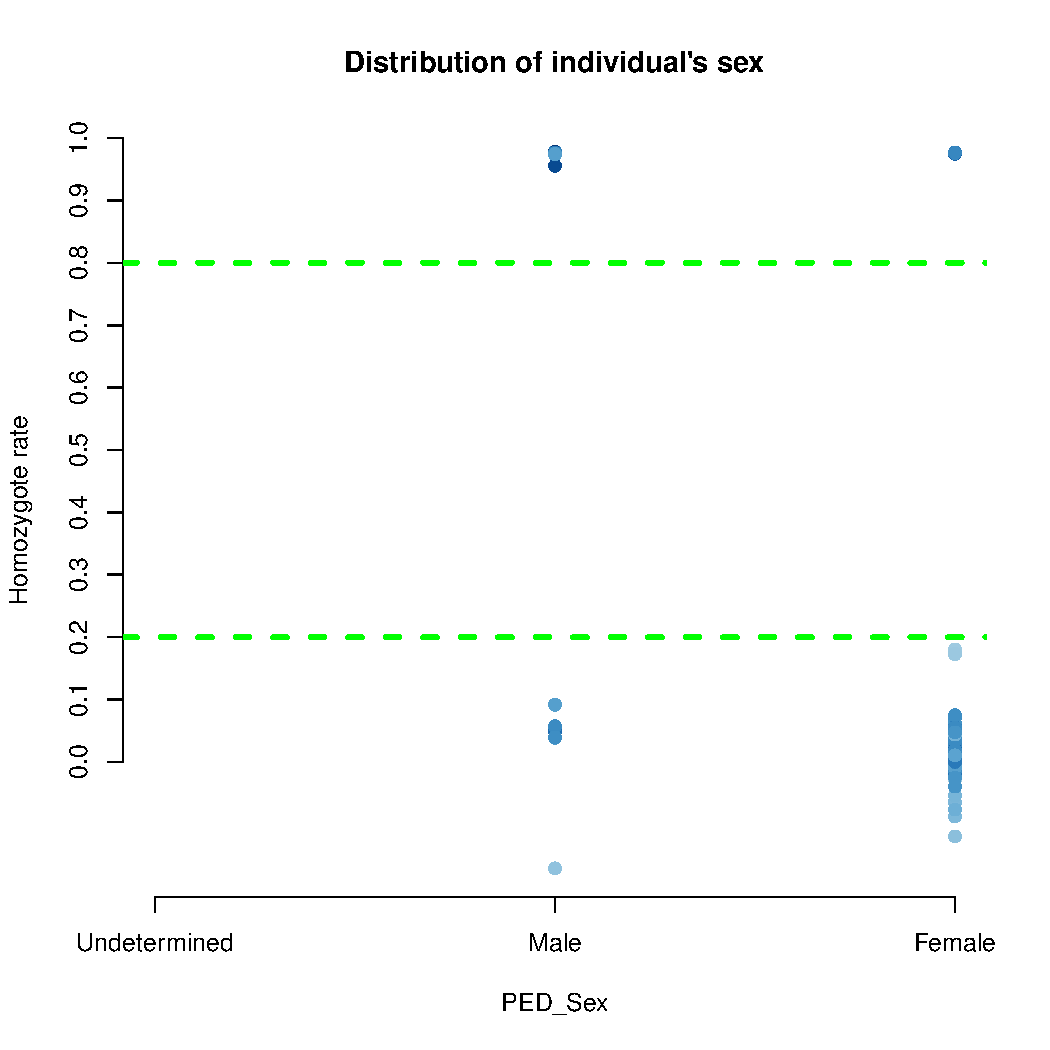
\includegraphics[width=0.6\textwidth]{/Users/chenchun-yu/QC/test/sex_distribution.pdf}
\centering
\caption{Distribution of individual's sex. When the homozygosity rate is more than 0.8, the sex of individuals will regard as male; in the other hand, indviduals will regard as female when the homozygosity rate is less than 0.2. When the homozygosity rate is more than 0.2 but less than 0.8, the genotype data are inconclusive regarding the sex of an individual.}
\end{figure}
\newpage
% latex table generated in R 3.2.1 by xtable 1.8-0 package
% Fri Jan 15 18:18:57 2016
\begin{table}[ht]
\centering
\caption{Sex information of 96 samples} 
\begin{tabular}{lcr}
  \hline
Sex & By SNP & By record \\ 
  \hline
Male & 38 & 45 \\ 
  Female & 47 & 51 \\ 
  PROBLEM & 11 & 0 \\ 
   \hline
\end{tabular}
\end{table}

\begin{table}[h]
\centering
\caption{Individuals with discordant sex information} 
\begin{tabular}{lr}
  \hline
Family ID & Individual ID \\ 
  \hline
6&TDC497 \\
8&TDC486 \\
13&TDC495 \\
18&TDC494 \\
29&TDC475 \\
31&TDC213 \\
58&TDC465 \\
65&TDC545 \\
79&TDC506 \\
80&TDC22 \\
82&TDC451 \\
   \hline
\end{tabular}
\end{table}
\subsubsection{Distribution of missingness and heterozygosity scores}
Missing data rates and heterozygosity rate were measured to identify individuals with low DNA sample quality. In our results, there were 2 individuals out of our threholds. Specifically, sample 18 was reported by genome center that it might contaminate during genotyping.
\begin{figure}[h]
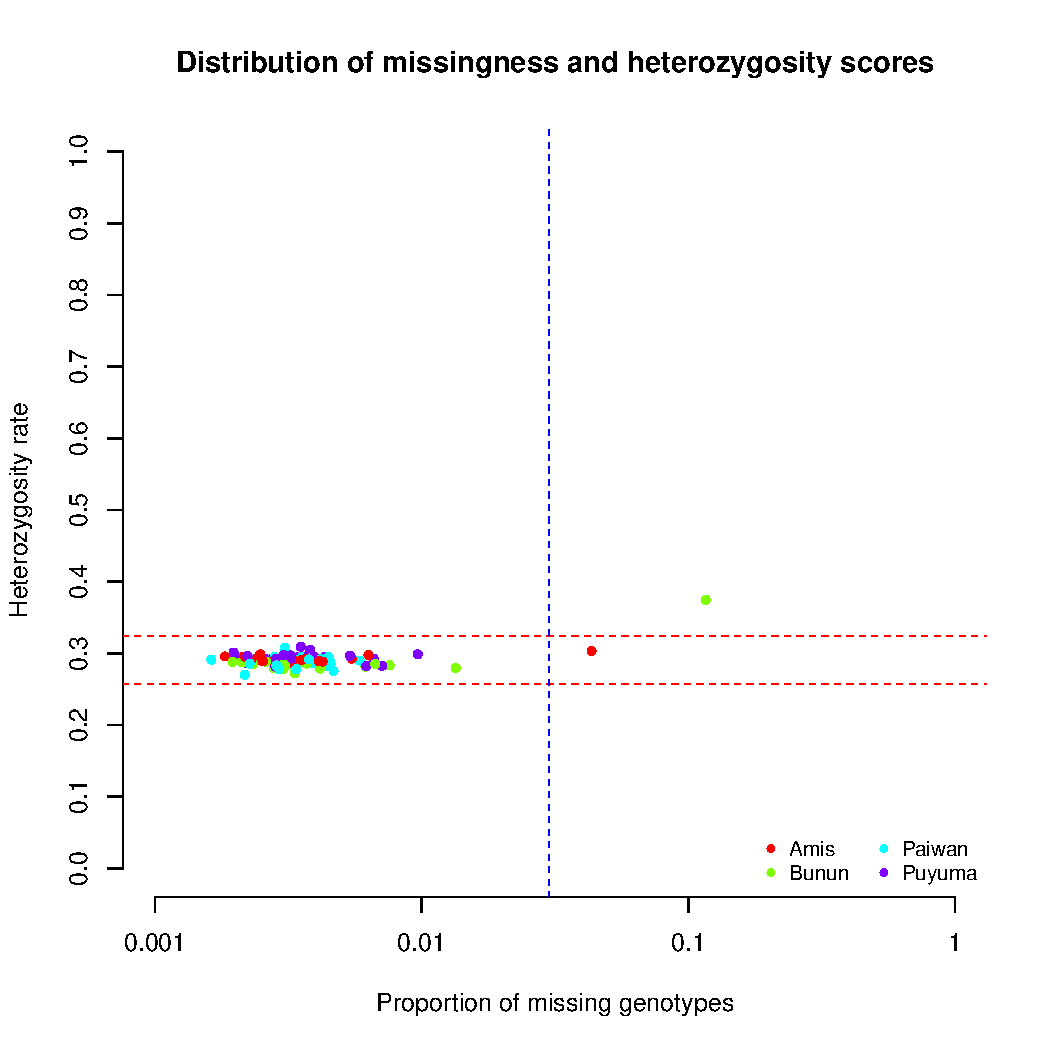
\includegraphics[width=0.6\textwidth]{/Users/chenchun-yu/QC/test/imiss-vs-het.pdf}
\centering
\caption{Distribution of missingness and heterozygosity scores. We chose to exclude all individuals with a genotype failure rate ≥0.03 and/or a heterozygosity rate ± 3 s.d. from the mean.}
\end{figure}
\newpage
% latex table generated in R 3.2.1 by xtable 1.8-0 package
% Fri Jan 15 18:15:53 2016
\begin{table}[h]
\centering
\caption{Individuals with high missingness and/or outlier heterozygosity} 
\begin{tabular}{lr}
  \hline
Family ID & Individual ID \\ 
  \hline
 18 & TDC494 \\ 
   73 & TDC489 \\ 
   \hline
\end{tabular}
\end{table}

\subsubsection{Propotion of the different IBD}
To remove related individuals, we set IBD value of 0.18575 as criteria. The IBD value of 0.1875 was calculated from (0.125 + 0.25 )/2 which 0.125 refered to third-degree relatives and 0.25 represented for second-degree relatives. In our results, there were 8 individuals which IBD were lager than 0.1875. Those individuals not only related to some individuals in samples but with lower call rates which stored in 96smples.imiss.
\begin{figure}[h]
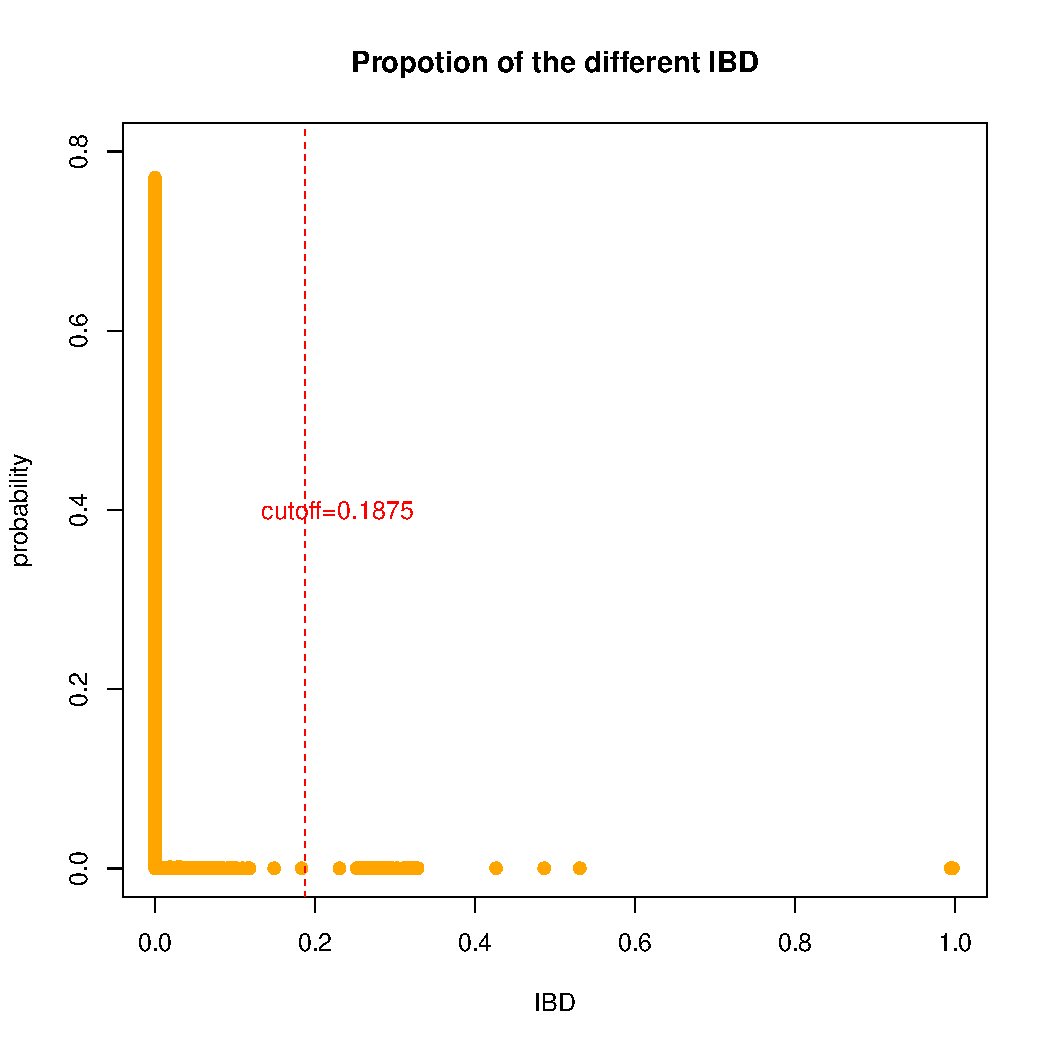
\includegraphics[width=0.6\textwidth]{/Users/chenchun-yu/QC/test/ibd.pdf}
\centering
\caption{Propotion of the different IBD. Verticle lines show the threhold with IBD equals to 0.1875.}
\end{figure}
\newpage
\begin{table}[h]
\centering
\caption{Individuals with high IBD} 
\begin{tabular}{lr}
  \hline
Family ID & Individual ID \\ 
  \hline
18&TDC494 \\
22&TDC500 \\
25&TDC165 \\
28&TDC406 \\ 
36&TDC478 \\
56&TDC480-2 \\
74&TDC212 \\
89&TDC480 \\
   \hline
\end{tabular}
\end{table}
\subsection{Per-marker QC}
\subsubsection{Distribution of excessive missing data rate}
\newpage
\begin{figure}[h]
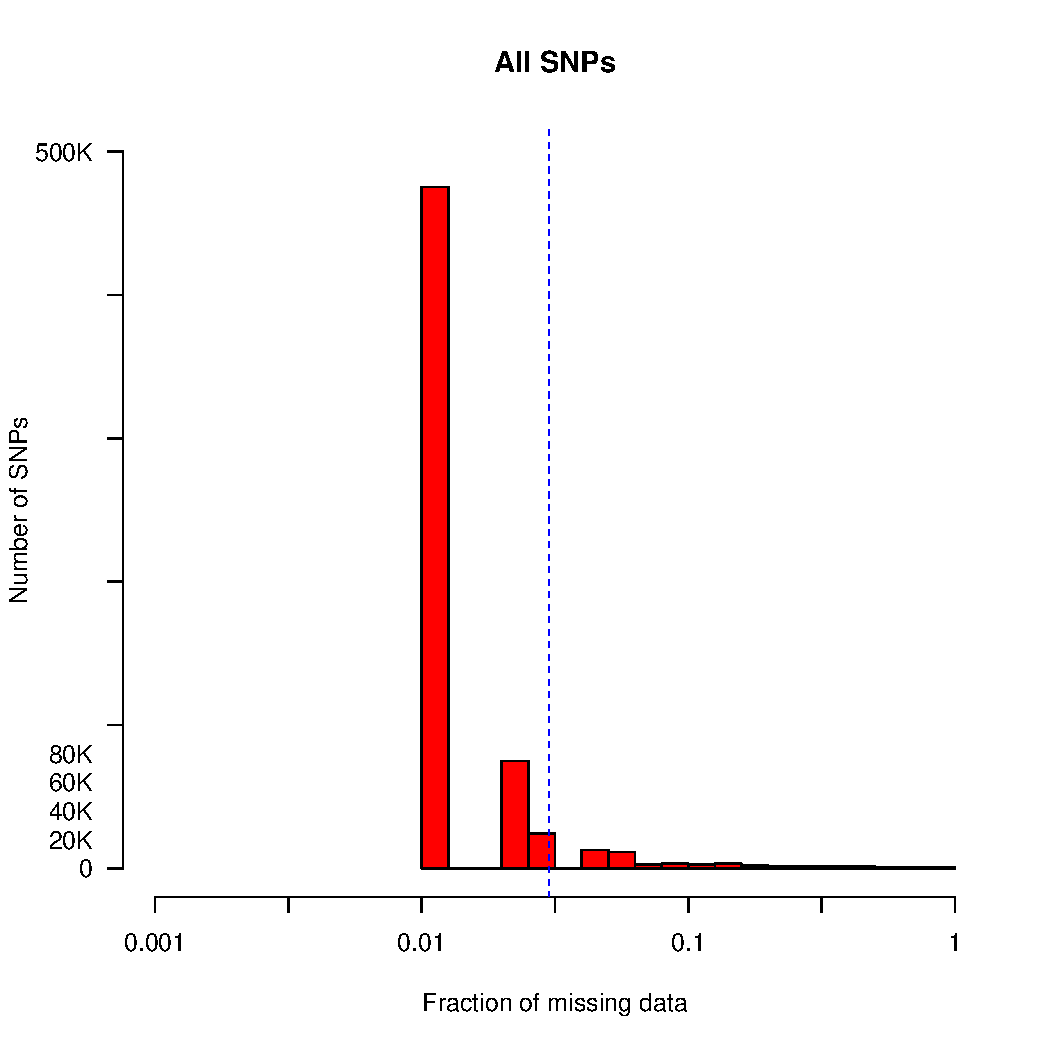
\includegraphics[width=0.6\textwidth]{/Users/chenchun-yu/QC/test/hist_missing_geno.pdf}
\centering
\caption{Histogram of missing data rate across all individuals passing ‘per-individual’ quality control. The dashed vertical line represents the threshold (3\%) at which SNPs were removed from further analysis because of an excess failure rate.}
\end{figure}
\newpage
\begin{figure}[h]
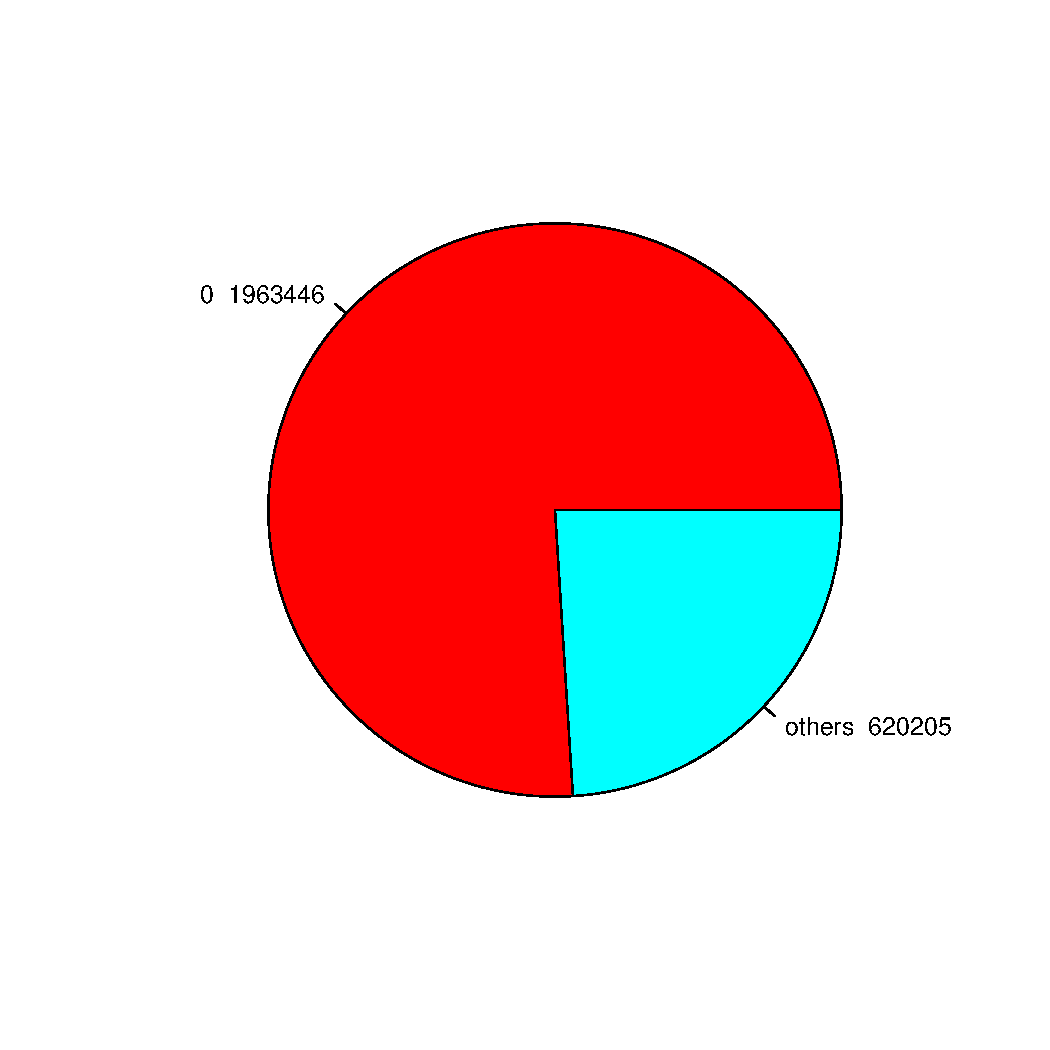
\includegraphics[width=0.6\textwidth]{/Users/chenchun-yu/QC/test/pie_missing_geno.pdf}
\centering
\caption{Pie chart shows the propotion of missing genotype rate = 0 and IBD\textgreater 0. The proportions of IBD=0 is about 76\%; IBD\textgreater 0 is about 24\%.}
\end{figure}
\section{References}
1. Anderson et al. Data quality control in genetic case-control association studies, Nature protocols, 2010.
\end{document}
